\section{Bases and dimension}

A linearly independent generating set for \textit W possesses a very useful property-every vector in \textit W can be expressed in one and only one way as a linear combination of the vectors in the set. It's this property that makes linearly independent generating sets the building blocks of vector spaces.

\dfn{}{
  A \textbf{basis} $\beta$ for a vector space \textit V is a linearly independent subset of \textit V that generates \textit V. If $\beta$ is a basis for \textit V, we also say that the vectors of $\beta$ form a basis for \textit V.
}

The next theorem, which is used frequently in Chapter 2, establishes the most significant property of a basis.

\thm{}{
  Let \textit V be a vector space and $\beta = \{u_1, u_2, \cdots, u_n\} \subseteq V$. Then $\beta$ is a basis for \textit V if and only if each $v \in V$ can be uniquely expressed al a linear combination of vectors of $\beta$, that is, can be expressed in the form $$v = \lambda_1 u_1 + \lambda_2 u_2 + \cdots + \lambda_n u_n$$ for unique scalars $\lambda_1, \lambda_2, \cdots, \lambda_n$
}

We're primarily interested in vector spaces having finite bases. The next theorem identifies a large class of vector spaces of this type.

\thm{}{
  If a vector space \textit V is generated by a finite set \textit S, then some subset of \textit S is a basis for \textit V. Hence \textit V has a finite basis.
}

The corollaries of the following theorem are perhaps the most significant results in the current Chapter.

\thm{Replecement Theorem}{
  Let \textit V be a vector space that's generated by a set \textit G containing exactly \textit n vectors, and let \textit L be a linearly independent subset of \textit V containin exactly \textit m vectors. Then $m \le n$ and there exists a subset $H \subseteq G$ containing exactly $n - m$ vectors such that $L \cup H$ generates \textit V.
}

\cor{}{
  Let \textit V be a vector space having a finite basis. Then every basis for \textit V contains the same number of vectors.
}

If a vector space has a finite basis, the preceding corollary asserts that the number of vectors in \textit{any} basis for \textit V is an intrinsic property of \textit V. This fact makes possible the following important definitions.

\dfn{}{
  A vector space is called \textbf{finite-dimensional} if it has a basis consisting of a finite number of vectors. The unique number of vectors in each basis for \textit V i called the \textbf{dimension} of \textit V and is denoted by dim(\textit V). A vector space that isn't finite-dimensional is called \textbf{infinite-dimensional}.
}

\newpage
Just as no linearly independent subset of a finite-dimensional vector space \textit V can contain more than dim(\textit V) vectors, a corresponding statement can be made about the size of a generating set.

\cor{}{
  Let \textit V be a vector space with dimension \textit n.
  \begin{enumerate}[a)]
    \item Any finite generating set for \textit V contains at least \textit n vectors, and a generating set for \textit V that contains exactly \textit n vectors is a basis for \textit V.
    \item Any linearly independent subset of \textit V that contains exactly \textit n vectors if a basis for \textit V.
    \item Every linearly independent subset of \textit V can be extended to a basis for \textit V.
  \end{enumerate}
}

\subsection{An Overview of Dimension and Its consequences}

Let's summarize here the main results of this section in order to put them into better perspective.

A basis for a vector space \textit V is a linearly independent subset of \textit V that generates \textit V. If \textit V has a finite basis, then every basis for \textit V contains the same number of vectors. This number is called the  dimension of \textit V, and \textit V is said to be finite-dimensional. Thus if the dimension of \textit V is \textit n, every basis for \textit V contains exactly \textit n vectors. Moreover, every linearly independent subset of \textit V contains no more than \textit n vectors and can be extended to a basis for \textit V by including appropiately chosen vectors. Also, each generating set for \textit V contains at least \textit n vectors and can be reduced to a basis for \textit V by excluding appropiately chosen vectors.
\begin{center}
  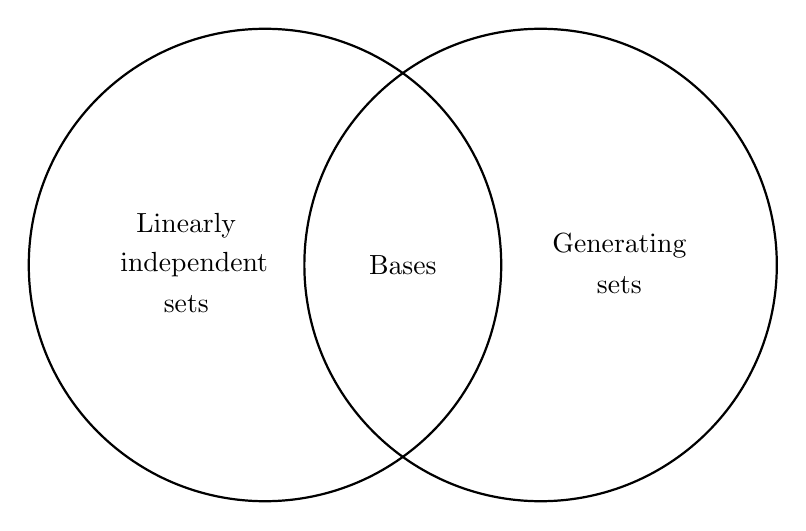
\begin{tikzpicture}
      % Define the radius of the circles
      \def\radius{3cm}
      
      % Draw the left circle (Linearly independent sets)
      \draw[thick] (0,0) circle (\radius);
      % Draw the right circle (Generating sets)
      \draw[thick] (3.5,0) circle (\radius);
      
      % Label the left circle
      \node at (-1,.5) {Linearly};
      \node at (-.9,0) {independent};
      \node at (-1,-.5) {sets};
      
      % Label the right circle
      \node at (4.5,.25) {Generating};
      \node at (4.5,-.25) {sets};
      
      % Label the overlapping section
      \node at (1.75,0) {Bases};
  \end{tikzpicture}
\end{center}


\subsection{The dimension of Subspaces}

Our next result relates the dimension of a subspace to the dimension of the vector space that contains it.

\thm{}{
  Let \textit W be a subspace of a finite-dimensional vector space \textit V. Then \textit W is finite-dimensional and dim(\textit W) $\le$ dim(\textit V). Moreover, if dim(\textit W) = dim(\textit V), then $V = W$.
}

\cor{}{
  If \textit W is a subspace of a finite-dimensional vector space \textit V, then any basis for \textit W can be extended to a basis for \textit V.
}
